\documentclass[12pt]{article}
%\usepackage{tkiz}

\usepackage[utf8]{inputenc}
\usepackage[french]{babel}
\usepackage{amsmath,amsthm,amsfonts,amssymb}
\usepackage{lmodern}
\usepackage[top=2.4cm,bottom=2.4cm,left=2cm,right=2cm]{geometry}
\usepackage{hyperref}
\usepackage{multicol}
\usepackage{enumitem}
\usepackage{listings}
\usepackage[dvipsnames]{xcolor}
\usepackage{tikz}

%\date{}
\title{{\bf  Génie logiciel} \\
	Notes du cours de 21/10 , partie 1 \\
	{\small L3 Informatique appliquée 2022-2023} \\
	{\it \small MABROUK Fayez}}
\begin{document}
	\maketitle
	\newpage
	\section{UML pour modéliser la dynamique}
	\subsection{La dynamique}
	\begin{itemize}
		\item [*] Nous avons vu un diagramme permettant de modéliser l'interaction entre des entités internes (système) et externes (acteur).
		\item[*] Comment interagissent-elles ?
		\item [*]Diagramme de séquence : modélisation des aspects temporels.
		\item[*] Diagramme de communication : modélisation des aspects spatiaux.
	\end{itemize}
\section{Diagramme de séquence}
\subsection{Diagramme de séquence}
\begin{itemize}
	\item[*] Un diagramme de séquence décrit les interactions entre différents objets en
	montrant les messages transmis entre eux.
	\item[*] Montre:
	\begin{itemize}
		\item[*] Comment les objets interagissent entre eux.
		\item [*] Quelles informations échangent-ils (facultatif).
		\item [*] Dans quel ordre communiquent-ils ?
		
	\end{itemize}
\item[*] Utilisez-le pour montrer comment les petites méthodes sont séquencées.
\item[*] Un cas d'utilisation doit être accompagné d'un diagramme de séquence.
\end{itemize}
\subsection{Ligne de vie d'un objet}
\begin{itemize}
	\begin{figure}[!hbtp]
		%\centering
		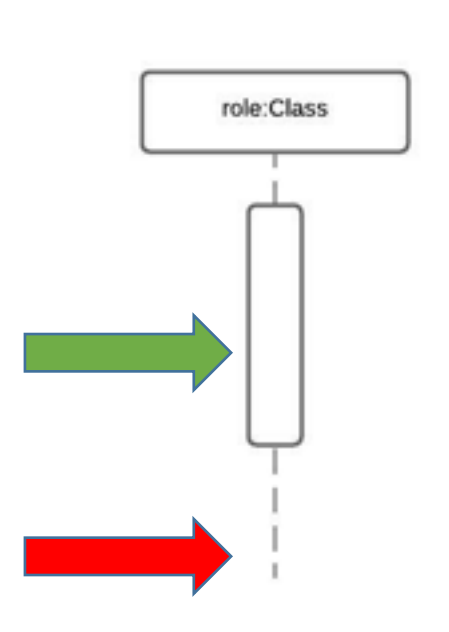
\includegraphics[scale=0.75]{Capture3.PNG}
		%\caption{Légende de l'image}
	\end{figure}
\item[*] Chaque instance d'un objet est nommée avec la notation
"rôle : Class". S'il n'y a pas d'ambiguïté, ":Class" peut être
suffisant.
\item[*] Chaque instance d'un objet possède une \textcolor{red}{ligne de vie}, représentée par un trait en
ligne en pointillés.
\item[*] Le diagramme se lit de haut en bas : le temps augmente
quand on descend.
\item[*] \textcolor{green}{La période d'activation} représente le temps pendant lequel
l'instance est active (c'est-à-dire qu'elle exécute une méthode).
\end{itemize}
\subsection{Envoi de messages}
\begin{itemize}
		\begin{figure}[!hbtp]
		%\centering
		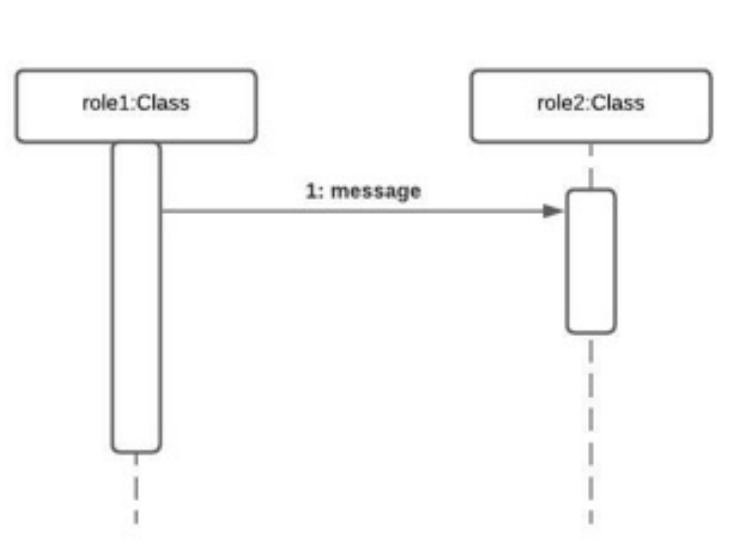
\includegraphics[scale=0.75]{Capture4.PNG}
		%\caption{Légende de l'image}
	\end{figure}
	\item [*] Flèche horizontale
	de la ligne de vie de l'expéditeur
	de l'expéditeur au
	récepteur.
	\item[*] Un message = 1
	numéro (en
	ordre séquentiel)
	+ un nom.
		\begin{figure}[!hbtp]
		%\centering
		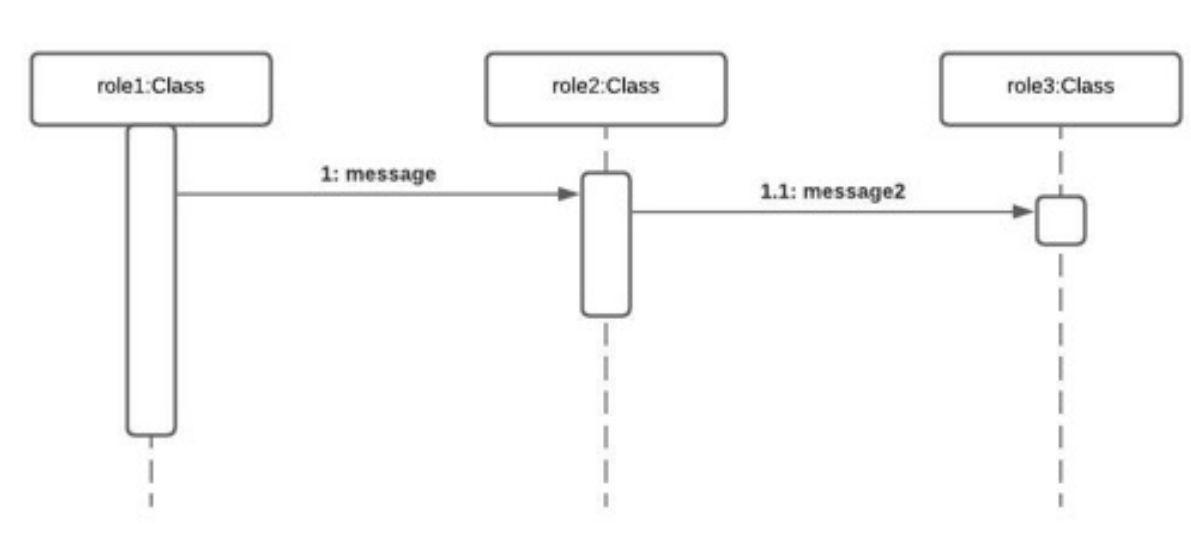
\includegraphics[scale=0.75]{Capture5.PNG}
		%\caption{Légende de l'image}
	\end{figure}
	\item[*] Flèche horizontale
	de la ligne de vie de l'expéditeur
	de l'expéditeur au
	récepteur.
	\item[*] Un message = 1
	numéro (en
	ordre séquentiel)
	+ un nom.
	\item[*] Lorsqu'un message
	est envoyé alors que le
	précédent n'est
	n'est pas terminé : sous numérotation.
	\\
	\\
	\item[*] Le message peut être:
	\begin{itemize}
		\item[*] Synchrone : l'expéditeur arrête son activité pendant que le destinataire travaille sur le message.
		\item[*] Asynchrone : l'expéditeur n'arrête pas son activité.
		\item[*] Réponse.
	\end{itemize}
\item[*] Possibilité d'envoyer un message à soi-même.
\\
\\
\item[*] Le message ne doit pas nécessairement porter un nom. Dans ce cas :
\\
\item[*] Le message peut intégrer des données par le biais de paramètres:
\\
\item[*] Les paramètres peuvent être omis par '-':
\\ 
\begin{figure}[!hbtp]
	%\centering
	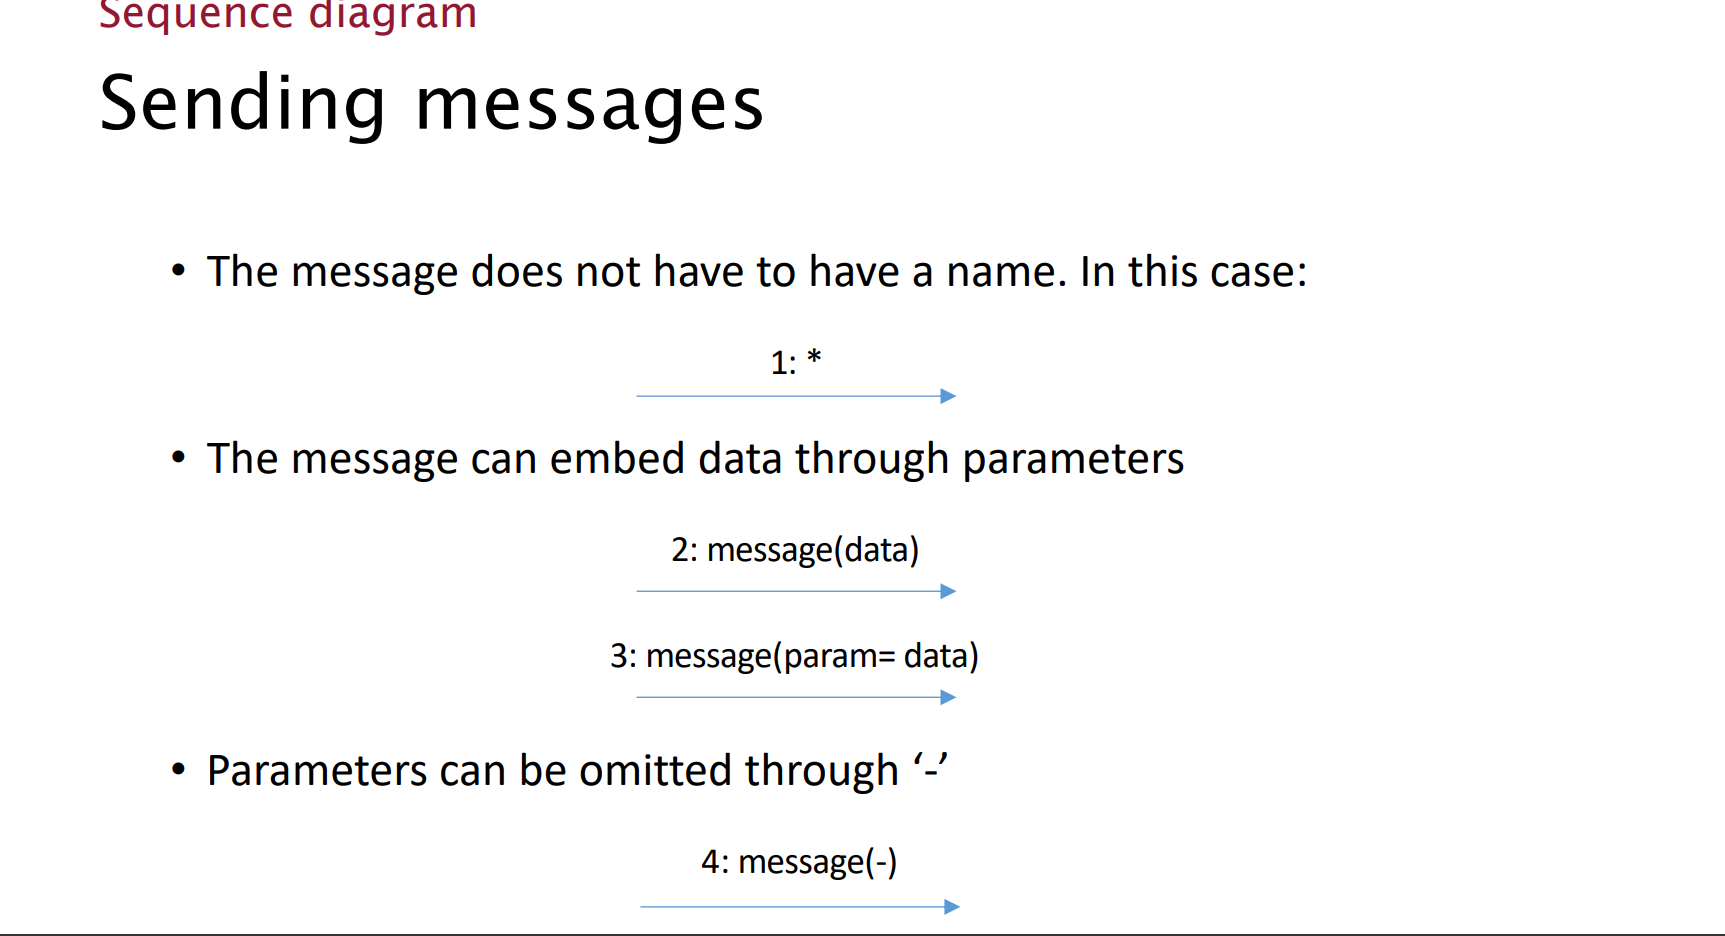
\includegraphics[scale=0.75]{Capture7.PNG}
	%\caption{Légende de l'image}
\end{figure}
\end{itemize}
\end{document}